\documentclass[border=8pt]{standalone}
\usepackage{amsmath}
\usepackage{fontspec}
\setmainfont{Source Serif 4}
\usepackage{pgfplots}
\pgfplotsset{compat=1.18}
\definecolor{qbase}{RGB}{31,86,160}
\definecolor{winner}{RGB}{209,73,91}

\begin{document}
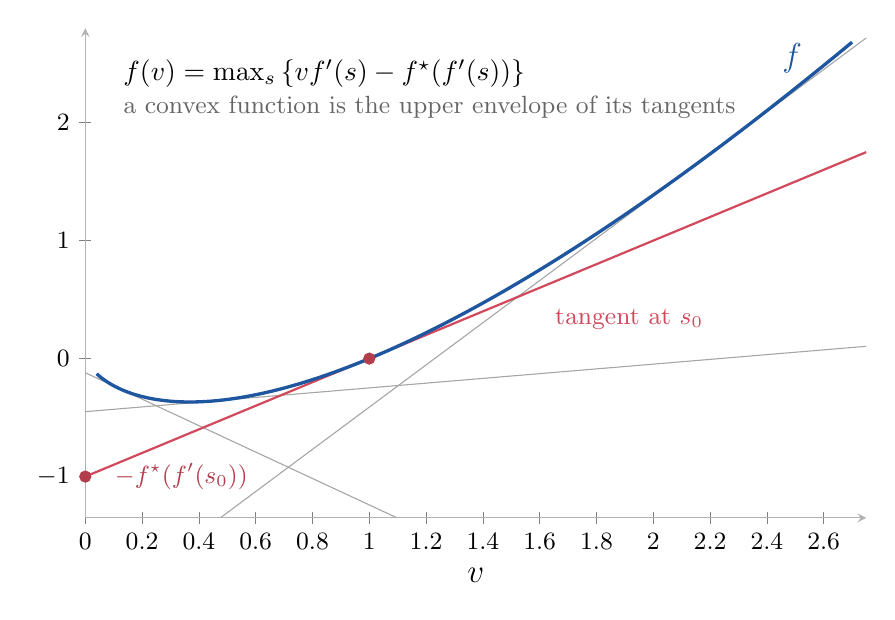
\begin{tikzpicture}
\begin{axis}[
  width=11.5cm, height=7.8cm,
  axis lines=left,
  xlabel={$v$},
  xmin=0, xmax=2.75, ymin=-1.35, ymax=2.8,
  ytick={-1, 0, 1, 2},
  label style={font=\large},
  tick label style={font=\small},
  axis line style={gray!60},
  clip=true,
]
% tangent lines at s in {0.12, 0.45, 2.2}: v*(ln s + 1) - s
\addplot[domain=0:2.75, samples=2, thin, black!35] {x*(ln(0.12)+1) - 0.12};
\addplot[domain=0:2.75, samples=2, thin, black!35] {x*(ln(0.45)+1) - 0.45};
\addplot[domain=0:2.75, samples=2, thin, black!35] {x*(ln(2.2)+1) - 2.2};
% highlighted tangent at s0 = 1: y = v - 1
\addplot[domain=0:2.75, samples=2, thick, winner] {x - 1};
% the convex function f(v) = v ln v
\addplot[domain=0.04:2.7, samples=200, very thick, qbase] {x*ln(x)};
% tangency point and intercept
\addplot[only marks, mark=*, mark size=2pt, winner!85!black] coordinates {(1,0)};
\addplot[only marks, mark=*, mark size=2pt, winner!85!black] coordinates {(0,-1)};
\node[winner!85!black, font=\small, anchor=west] at (axis cs:0.07,-1)
  {$-f^{\star}(f'(s_0))$};
\node[winner, font=\small, anchor=north west] at (axis cs:1.62,0.50)
  {tangent at $s_0$};
\node[qbase, font=\large, anchor=west] at (axis cs:2.42,2.55) {$f$};
% the identity
\node[font=\normalsize, anchor=north west, align=left] at (axis cs:0.1,2.62)
  {$f(v) = \max_{s} \left\{ v f'(s) - f^{\star}(f'(s)) \right\}$\\
   {\small\color{black!60} a convex function is the upper envelope of its tangents}};
\end{axis}
\end{tikzpicture}
\end{document}
